%%%%%%%%%%%%%%%%%%%%%%%%%%%%%%%%%%%%%%%%%%%%%%%%%%%%%%%%%%%%%%%%%%%%%%%%%%%%
% Section 2: Background Information of RapidSmith, RapidSmith2, and Tincr
%%%%%%%%%%%%%%%%%%%%%%%%%%%%%%%%%%%%%%%%%%%%%%%%%%%%%%%%%%%%%%%%%%%%%%%%%%%%
\newpage
\section{Vivado, RS2, and Tincr}
\subsection{RapidSmith vs. RS2}
\subsubsection{What Was The Original RapidSmith?}
The original RapidSmith was written by Christopher Lavin as a part of his PhD
work at BYU.  It was based on the Xilinx Design Language (XDL) which provides a
human-readable file format equivalent to the Xilinx proprietary Netlist Circuit
Description (NCD) of ISE.  With RapidSmith, researchers were able to import
XDL/NCD, manipulate, place, route and export designs among a variety of design
transformations.  The RapidSmith project made an excellent test bed to try out
new ideas and algorithms for FPGA CAD research because code could quickly be
written to take advantage of the APIs available.

RapidSmith also contained packages which could parse/export bitstreams (at the
packet level) and represent the frames and configuration blocks in the provided
data structures.  In this regard, RapidSmith did not include any proprietary
information about Xilinx FPGAs that is not publicly available.

RapidSmith continues to be functional and is still available at the
SourceForge.net website.  There, you will find documentation, installation
instructions, the RapidSmith code base, and a collection of demo programs based
on it.

\subsubsection{What is RS2?}
With the announced end of ISE (with the Virtex7 family of parts being the last
family to be supported by ISE), there was no path forward to newer parts using
RapidSmith.  This is because XDL is not available with Vivado. With
Vivado, however, Xilinx has provided an extensive Tcl scripting capability which 
initially looked as if it could provide a similar capability to that provided by
XDL in terms of accessing both Vivado's design and device data and in terms of
creating and modifying Vivado designs.  However, as described above, Vivado's
Tcl is limited by speed and memory challenges.
The development of RS2 consisted of three parts.

\subsubsection{Tincr: Integrating Custom CAD Tool Frameworks with the Xilinx 
Vivado Design Suite} \label{sec:tincr}

In the first part, the Vivado Tcl capability was investigated to ensure that,
indeed, it did provide the needed ability to access design and device data and
export that to external tools such as RapidSmith.  This resulted in the Tincr
project, led by Brad White as a part of his MS work at BYU, with Thomas
Townsend making additions as a part of his research.

Tincr is a Tcl-based library of routines which (a) provide a variety of
functions to simply make working with Vivado via Tcl easier, (b) provide a way
to export all the data associated with a Vivado design into what is called a
Tincr Checkpoint (TCP), (c) provide a way to reimport Tincr Checkpoints back
into Vivado, and (d) access device data from Vivado and output that data in the
form of XDLRC files (these are the files which XDL used to describe devices and
are necessary for RapidSmith and RS2 to understand the structure of and the
resources available for use in a given Xilinx part).  Tincr is available at 
\href{https://github.com/byuccl/tincr}{\color{blue}https://github.com/byuccl/tincr}.
Tincr is described in two publications:

\begin{quotation}B. White and B. Nelson, "Tincr — A custom CAD tool framework
for Vivado," 2014 International Conference on ReConFigurable Computing and FPGAs (ReConFig14),
Cancun, 2014, pp. 1-6, DOI: 10.1109/ReConFig.2014.7032560

White, Brad S., "Tincr: Integrating Custom CAD Tool Frameworks with
the Xilinx Vivado Design Suite" (2014), BYU Scholars Archive, Paper 4338. 
\\URL:http://scholarsarchive.byu.edu/etd/4338
\end{quotation}

\subsubsection{RS2: A Framework for BEL-Level CAD Exploration on Xilinx FPGAs}
The second part of the development of RS2 was to add a new layer of design
representation to RapidSmith which more closely matches that of Vivado.  This
was done as a part of his PhD work by Travis Haroldsen at BYU.  As of this
writing, one paper on RS2 has appeared:

\begin{quotation}Travis Haroldsen, Brent Nelson, and Brad Hutchings, “RapidSmith
2:
A Framework for BEL-Level CAD Exploration on Xilinx FPGAs�, Proceedings of the
2015 ACM/SIGDA International Symposium on Field-Programmable Gate Arrays,
February 2015, Monterey CA, pp. 66-69, DOI: 10.1145/2684746.2689085.
\end{quotation}

\subsubsection{Vivado and RS2 Integration}
The third part of the development of RS2 was to create the ability to export
designs from Vivado and into RS2 and, correspondingly, to import RS2 data back
into Vivado.  This was completed during 2016, largely by Thomas Townsend
as an MS student at Brigham Young University.  The initial
public release of RS2 was made in January 2017 once that piece was in place.

\subsubsection{What is All This About XDL and XDLRC and How Does RS2 Fit Into
That?} 
The Xilinx ISE tools had the capability to export XDL and XDLRC files which
RapidSmith used: 
\begin{itemize}
  \item An XDLRC file was a complete description of a given Xilinx FPGA,
  describing every tile, every switchbox, every wire segment, and every PIP in
  the part.  RapidSmith was able to process this information and create a device
  representation for use in support of CAD tools such as placers and routers.
  \item An XDL file was a textual representation of an NCD file (a user design).
  It described the user design as a collection of \cls{Instances} and \cls{Nets}. Instances
  correspond to things like {SLICEs}, {BRAMs}, {DSP48s}, and {IOBs}.  Instances could be
  placed onto \cls{Sites}. Additionally, Nets in XDL consisted of a list of
  \cls{Pins} (their logical connections) and an optional list of \cls{PIPs} (their physical
  routing connections).
\end{itemize}
In Vivado, however, designs are described as a collection of \cls{Cells} where a Cell
corresponds to things like LUTs, flip flops, etc.  A Cell may be placed
onto a \cls{BEL} object such as an ALUT or a BFF.  RS2 contains a new layer of
hierarchy in its design and device descriptions where Cells and BELs are first-class objects and
design manipulation is all done at the Cell/BEL level.

Also, Vivado Nets are described using directed routing strings rather than lists
of PIPs.  RS2 also contains a set of new classes to enable the representation
and manipulation of Nets in a format compatible with these routing strings.

Thus, using RS2, design manipulation is now done at the level of Cells and BELs
and importing/exporting designs to/from Vivado is now fully supported.

\subsection{RS2 Usage Model and Structure}
The usage model for RS2 is shown in \autoref{fig:UsageModels}.  As can be
seen, a design can be exported from Vivado at multiple different points in the
Vivado design flow.  In each case, Tincr is used to export a Tincr Checkpoint
which can then be imported into RS2.  At those same points in the design flow,
RS2 can export a Tincr Checkpoint which can then be imported back into Vivado. 
Thus, a complete solution involves Vivado, Tincr, and RS2.

\begin{figure}[htb]
\centering
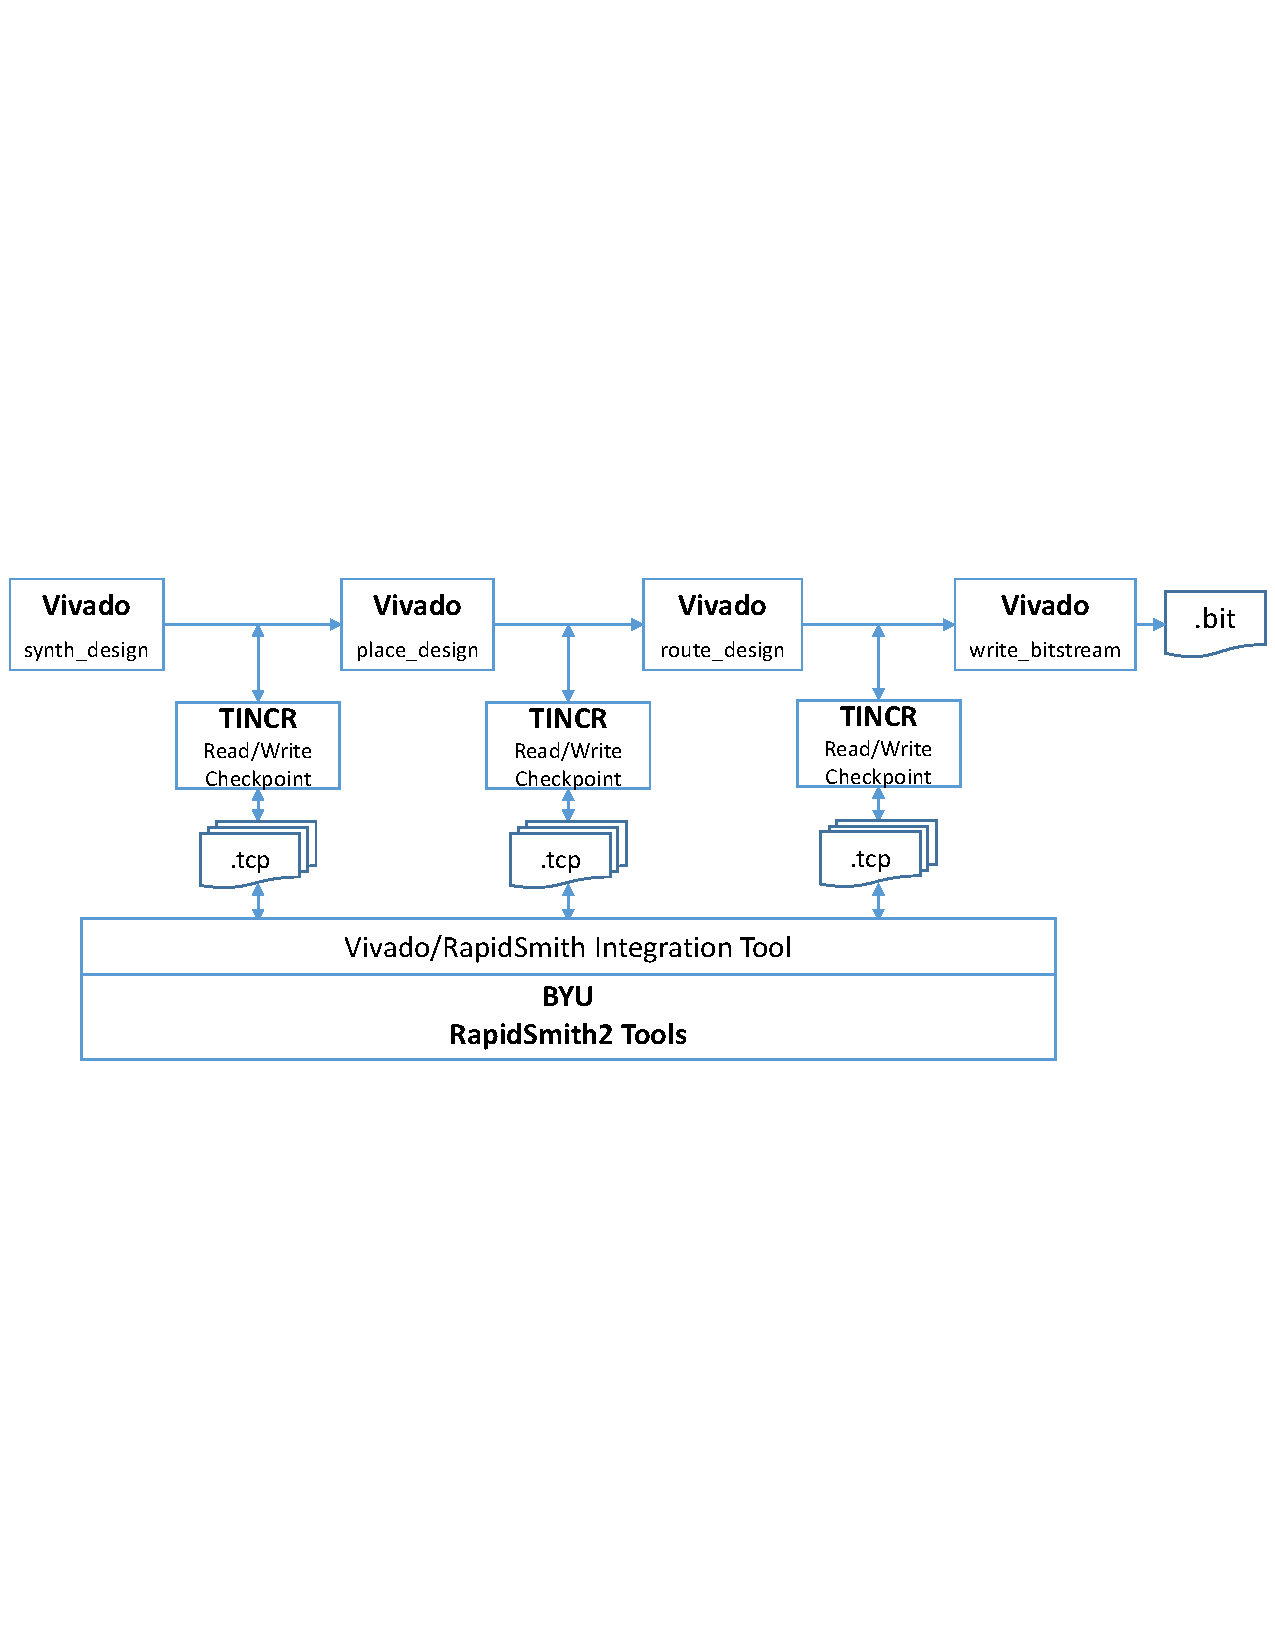
\includegraphics[width=\columnwidth]{UsageModels}
\caption{Vivado and RS2 Usage Model}
\label{fig:UsageModels}
\end{figure} 
